% =============================================================================
\section{Nivel 3: ver con cámara}
% =============================================================================

\begin{frame}{Separar percepción de control}
  \centering
  \begin{tikzpicture}[node distance=0.6cm,every node/.style={font=\scriptsize},
      bx/.style={draw=azul,fill=azulclaro,rounded corners,minimum height=0.7cm,align=center}]
    \node[bx,fill=gray!15,draw=gray] (gz) {Gazebo\\cámara};
    \node[bx,right=of gz,fill=gray!15,draw=gray] (br) {ros\_gz\_bridge};
    \node[bx,right=of br,fill=yellow!20] (det) {detector\_aruco\\(percepción)};
    \node[bx,right=of det,fill=yellow!20] (mis) {caza\_objetivo /\\estacion\_carga};
    \node[bx,right=of mis,fill=gray!15,draw=gray] (px) {PX4};
    \draw[-{Stealth}] (gz) -- (br);
    \draw[-{Stealth}] (br) -- node[above,font=\tiny,align=center]{/x500/camera/\\image} (det);
    \draw[-{Stealth}] (det) -- node[above,font=\tiny]{/x500/aruco} (mis);
    \draw[-{Stealth}] (mis) -- node[above,font=\tiny]{setpoints} (px);
  \end{tikzpicture}
  \vspace{0.6em}
  \begin{idea}
    \small El detector \textbf{no sabe nada de PX4 ni de misiones}; las misiones \textbf{no saben nada de
    OpenCV}. Si mañana cambian la cámara, el detector o el marcador, las misiones no se tocan. Las
    misiones 6 y 7 usan el mismo detector.
  \end{idea}
\end{frame}

\begin{frame}{ArUco en 1 lámina}
  \begin{columns}[c]
    \column{0.3\textwidth}\centering
    
\includegraphics[width=0.85\linewidth]{aruco_7}\\
    {\scriptsize id 7, DICT\_5X5\_250}
    \column{0.67\textwidth}\small
    \begin{itemize}
      \item Un cuadrado negro con una rejilla de 5\,$\times$\,5 celdas: el patrón codifica un \textbf{número}.
      \item \textbf{Diccionario} DICT\_5X5\_250: 250 patrones (ids 0--249), los de TMR y de \cmd{tools/aruco}.
      \item Necesita un \textbf{margen blanco} alrededor (zona quieta): sin él, sobre fondo oscuro no se
        encuentra la orilla.
      \item El detector da el id y las \textbf{4 esquinas} en píxeles.
    \end{itemize}
    \vspace{0.3em}
    \centering\scriptsize
    \begin{tabular}{lll}
      \toprule
      id & Dónde & Tamaño \\
      \midrule
      7 & techo de la camioneta sospechosa & 1.2 m \\
      3, 12, 25 & coches estacionados (señuelos) & 1.2 m \\
      42 & estación de carga & 1.4 m \\
      \bottomrule
    \end{tabular}
  \end{columns}
\end{frame}

\begin{frame}{El modelo de cámara (pinhole)}
  \begin{columns}[c]
    \column{0.5\textwidth}\centering
    \begin{tikzpicture}[scale=0.9]
      \draw[thick] (-2,0) -- (2,0) node[right,font=\tiny] {imagen};
      \fill (0,-1.6) circle (2pt) node[below,font=\tiny] {cámara};
      \draw[dashed] (0,-1.6) -- (0,0.4) node[above,font=\tiny] {$c_x$};
      \draw[azul,thick] (0,-1.6) -- (1.6,1.6);
      \fill[azul] (0.8,0) circle (2pt) node[above left,font=\tiny] {$u$};
      \draw[decorate,decoration={brace,mirror,amplitude=3pt}] (0,-0.1) -- (0.8,-0.1) node[midway,below=3pt,font=\tiny] {$u - c_x$};
      \draw[decorate,decoration={brace,amplitude=3pt}] (-0.1,-1.6) -- (-0.1,0) node[midway,left=3pt,font=\tiny] {$f_x$};
    \end{tikzpicture}
    \column{0.47\textwidth}\small
    \cmd{camera\_info} trae la matriz $K$: $f_x, f_y$ (focal en píxeles) y $c_x, c_y$ (centro).
    \[ x_n = \frac{u - c_x}{f_x} \qquad y_n = \frac{v - c_y}{f_y} \]
    $x_n$ es la \textbf{tangente del ángulo} del rayo desde el centro. A una altura $h$:
    \[ \text{desplazamiento} \approx x_n \cdot h \]
  \end{columns}
\end{frame}

\begin{frame}[fragile]{Los mensajes propios}
  \begin{columns}[t]
    \column{0.5\textwidth}
    \begin{lstlisting}[language=yaml,caption={msg/Aruco.msg}]
int32 id
float32 u          # [px] centro
float32 v          # [px]
float32 x_norm     # (u - cx) / fx
float32 y_norm     # (v - cy) / fy
float32 size_px    # [px] lado
    \end{lstlisting}
    \column{0.47\textwidth}
    \begin{lstlisting}[language=yaml,caption={msg/ArucoArray.msg}]
std_msgs/Header header
uint32 width       # [px]
uint32 height
Aruco[] markers    # vacía si no ve nada
    \end{lstlisting}
  \end{columns}
  \small Se generan con \cmd{rosidl\_generate\_interfaces} en el \cmd{CMakeLists.txt} (como en la intro a
  ROS 2: interfaces y \cmd{rosidl}). En C++: \cmd{\#include "x500\_retos/msg/aruco\_array.hpp"}.
\end{frame}

\begin{frame}[fragile]{detector\_aruco: tu parte}
  \begin{lstlisting}[style=cpp,caption={OpenCV 4.6 (el de Ubuntu 24.04): API cv::aruco::detectMarkers}]
cv_bridge::CvImageConstPtr gray = cv_bridge::toCvShare(msg, "mono8");  // ROS -> OpenCV, gris
const double fx = info_->k[0], cx = info_->k[2], fy = info_->k[4], cy = info_->k[5];
std::vector<int> ids;
std::vector<std::vector<cv::Point2f>> corners;
// TODO: detectar y llenar out.markers.
//   1. cv::aruco::detectMarkers(gray->image, dictionary_, corners, ids, params_);
//   2. Para cada uno: id, el centro (promedio de las 4 esquinas), x_norm, y_norm
//      y size_px (promedio de los 4 lados; cv::norm(a - b)).
  \end{lstlisting}
  \begin{ojo}
    \small En OpenCV 4.7+ la API cambió a \cmd{cv::aruco::ArucoDetector}. Los tutoriales nuevos no
    compilan con el OpenCV de Ubuntu 24.04.
  \end{ojo}
\end{frame}

\begin{frame}[fragile]{Ver lo que ve el detector}
  \begin{lstlisting}[style=bash]
ros2 run rqt_image_view rqt_image_view /x500/aruco/debug
ros2 topic echo /x500/aruco --field markers
  \end{lstlisting}
  \small
  \begin{itemize}
    \item \cmd{/x500/aruco/debug}: la imagen con los marcadores dibujados. Solo se publica si alguien la ve
      (dibujar cuesta).
    \item El detector procesa como mucho \cmd{max\_rate} = 15 imágenes por segundo.
    \item Para probarlo sin volar: \cmd{tools/render\_world.py} saca fotos de arriba de cualquier mundo; pásenle
      OpenCV en Python a esas fotos.
  \end{itemize}
\end{frame}

\begin{frame}{De un píxel a metros: la imagen}
  \begin{columns}[c]
    \column{0.45\textwidth}\centering
    \begin{tikzpicture}[scale=0.8]
      \draw[thick] (0,0) rectangle (4,3);
      \draw[-{Stealth},verde,thick] (2,1.5) -- (2,2.7) node[above,font=\tiny] {adelante (frente del dron)};
      \draw[-{Stealth},rojo,thick] (2,1.5) -- (3.4,1.5) node[right,font=\tiny] {derecha};
      \draw[-{Stealth},gray] (0,3) -- (0.8,3) node[above,font=\tiny] {u};
      \draw[-{Stealth},gray] (0,3) -- (0,2.2) node[left,font=\tiny] {v};
    \end{tikzpicture}
    \column{0.52\textwidth}\small
    La cámara mira hacia abajo. \textbf{Arriba de la imagen = el frente del dron}, derecha = derecha.
    Con el dron nivelado y a $h$ metros sobre el marcador:
    \[ \text{derecha} = x_n\,h \qquad \text{adelante} = -y_n\,h \]
    ($v$ crece hacia abajo de la imagen = hacia atrás del dron) y luego se rota por el heading a NED.
  \end{columns}
\end{frame}

\begin{frame}{Pero la cámara no tiene gimbal}
  \begin{columns}[c]
    \column{0.45\textwidth}\centering
    \begin{tikzpicture}[scale=0.85]
      \draw[thick] (-2.5,0) -- (2.5,0);
      \begin{scope}[shift={(0,3)},rotate=-15]
        \draw[thick,fill=gray!30] (-0.6,-0.08) rectangle (0.6,0.08);
        \draw[azul,dashed] (0,0) -- (0,-3.1);
      \end{scope}
      \draw[gray,dashed] (0,3) -- (0,0);
      \fill[rojo] (0,0) circle (2pt) node[below,font=\tiny] {debajo};
      \fill[azul] (0.8,0) circle (2pt) node[below,font=\tiny] {lo que ve al centro};
      \node[font=\tiny] at (1.3,3.2) {15°};
    \end{tikzpicture}
    \column{0.52\textwidth}\small
    Para acelerar, el dron se inclina. La cámara se inclina con él:
    \[ 12\text{ m} \cdot \tan 15° \approx 3.2\text{ m de error} \]
    Persiguiendo una camioneta eso hacía brincar la posición estimada y el seguimiento se perdía.
    \begin{idea}
      \small Solución (ya hecha en \cmd{aruco\_tools.hpp}): girar el rayo con la actitud \textbf{completa}
      del dron (cuaternión de PX4) y alargarlo hasta que baje $h$ metros.
    \end{idea}
  \end{columns}
\end{frame}

\begin{frame}[fragile]{El rayo con la actitud}
  \small En el cuerpo (FRD) el rayo del marcador es $\mathbf{r}_b = (-y_n,\ x_n,\ 1)$. Con la actitud $q$:
  \[ \mathbf{r}_{NED} = R(q)\,\mathbf{r}_b \qquad t = \frac{h}{r_{NED,z}} \qquad
     \Delta N = t\,r_{NED,x},\quad \Delta E = t\,r_{NED,y} \]
  \begin{lstlisting}[style=cpp,caption={Así se usa (ya está en las misiones)}]
const double height = -l.z - marker_h_;                // cámara sobre el marcador
const auto off = x500::marker_offset_ned(m, height, px4_.attitude().q);
const double n = l.x + off[0], e = l.y + off[1];        // el marcador en NED
  \end{lstlisting}
  \footnotesize Si el rayo casi no baja (dron muy inclinado), la función regresa (0, 0): no hay que confiar en esa vista.
\end{frame}

% ----------------------------------------------------------------------------- 6
\begin{frame}{Misión 6: la caza del objetivo}
  \begin{columns}[c]
    \column{0.5\textwidth}
    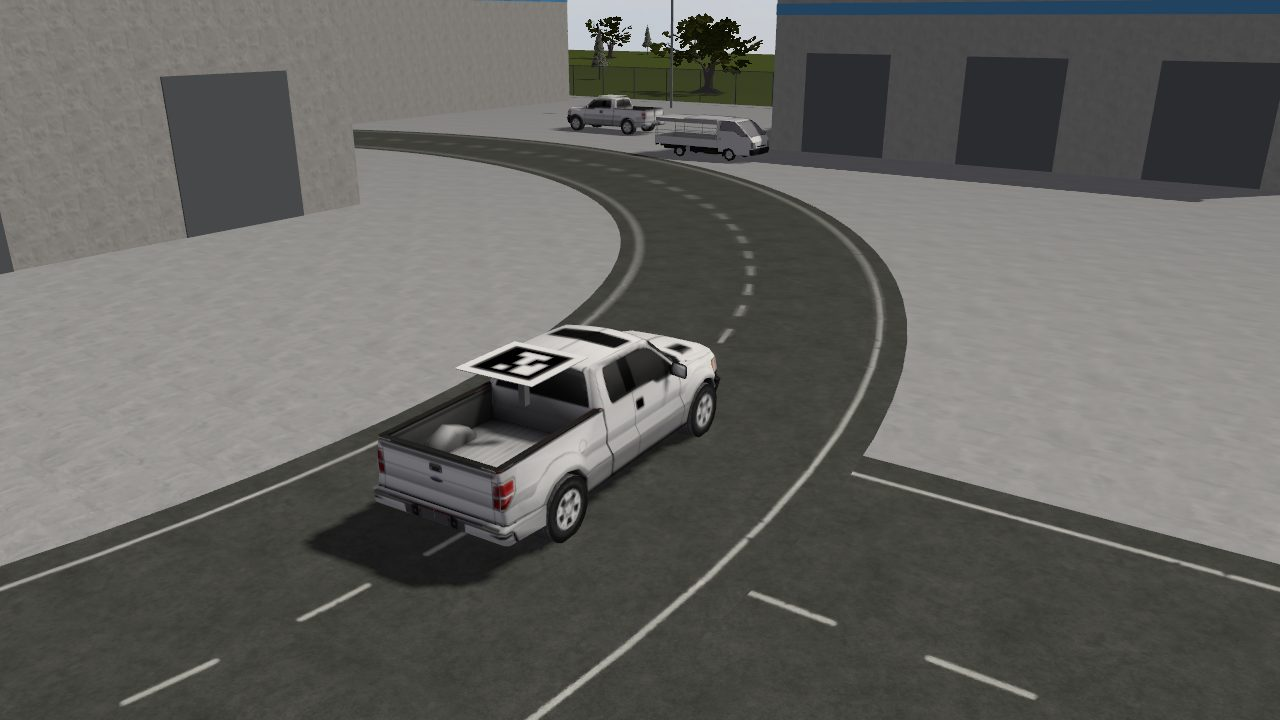
\includegraphics[width=\linewidth]{zona_bodegas_camioneta}
    \column{0.47\textwidth}\small
    \textbf{Escenario}: una camioneta sospechosa da vueltas en una zona de bodegas. Hay que
    \textbf{encontrarla}, \textbf{identificarla} por el ArUco 7 de su techo (no los señuelos),
    \textbf{dar su ubicación GPS} y \textbf{seguirla} desde arriba.
    \begin{itemize}
      \item Va a 3 m/s, una vuelta cada 55 s.
      \item \textbf{Lo nuevo}: perseguir algo que se \textbf{mueve}.
    \end{itemize}
  \end{columns}
\end{frame}

\begin{frame}{Buscar: el barrido ``podadora''}
  \begin{columns}[c]
    \column{0.47\textwidth}\centering
    \begin{tikzpicture}[x=0.045cm,y=0.045cm]
      \draw[gray!50,fill=gray!10] (-55,-12) rectangle (55,85);
      \draw[gray!60,line width=4pt,opacity=0.5] (0,42) circle (26.5);
      \draw[azul,thick,-{Stealth}] (-37.5,0) -- (-37.5,78) -- (-12.5,78) -- (-12.5,0) -- (12.5,0) -- (12.5,78) -- (37.5,78) -- (37.5,0);
      \draw[azul!30,line width=0.1pt,fill=azul!8,opacity=0.5] (-55,30) rectangle (-20,56);
      \node[font=\tiny,azul] at (-37.5,60) {ve};
      \node[draw,circle,fill=azulclaro,inner sep=0.5pt,font=\tiny] at (0,0) {H};
      \node[font=\tiny] at (0,42) {anillo};
    \end{tikzpicture}
    \column{0.5\textwidth}\small
    A 15 m, con 100° de campo, la cámara ve
    \[ 2\,h\tan(50°) \approx 36\ \text{m de ancho} \]
    Carriles norte--sur cada 25 m (se traslapan un poco) cubren todo el patio.
    \vspace{0.3em}

    Entre carriles avanza a \cmd{search\_speed} (5 m/s) con un punto que va 1 s adelante del dron y
    la velocidad como feedforward: si va muy rápido la cámara no alcanza a ver.
  \end{columns}
\end{frame}

\begin{frame}{Señuelos: filtrar por id}
  \begin{columns}[c]
    \column{0.45\textwidth}\centering
    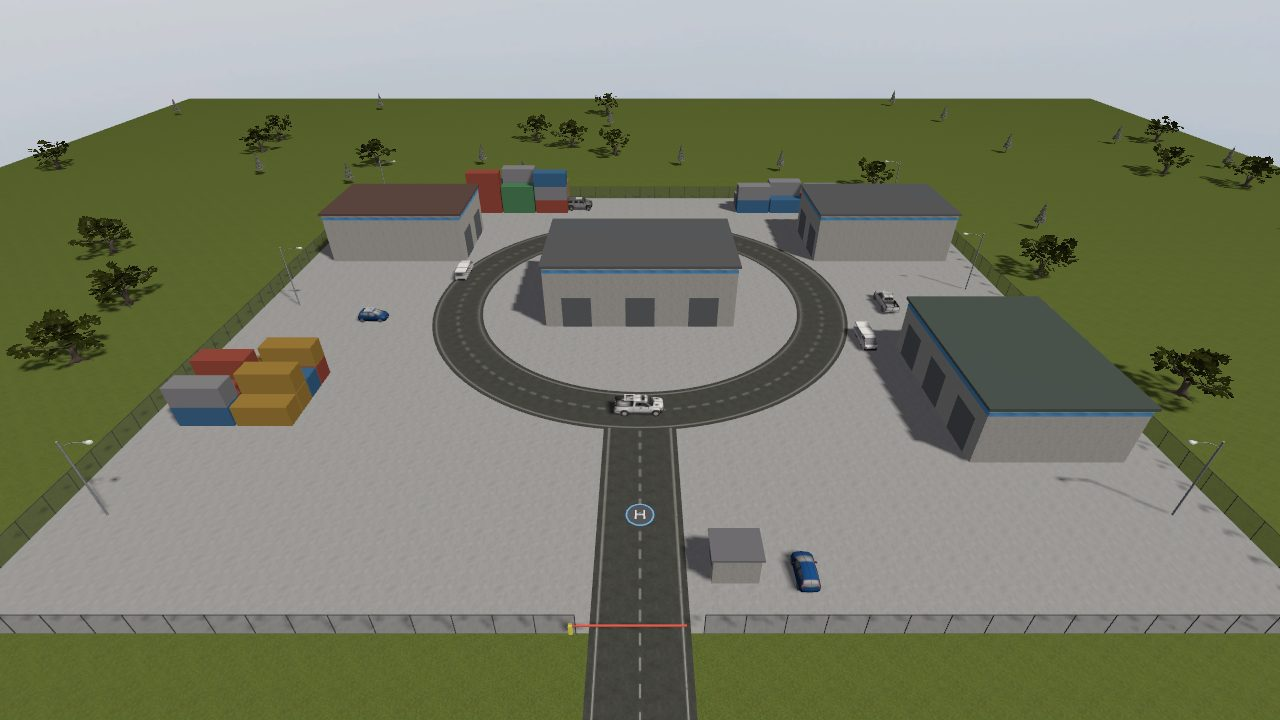
\includegraphics[width=0.9\linewidth]{zona_bodegas}
    \column{0.52\textwidth}\small
    Los coches estacionados también llevan ArUco (3, 12 y 25). El nodo los anuncia una vez y los ignora:
    \begin{terminal}{caza\_objetivo}
Veo el ArUco 3: es un señuelo, lo ignoro\\
Veo el ArUco 25: es un señuelo, lo ignoro\\
¡OBJETIVO ENCONTRADO! ArUco 7 en NED\\
\ norte 62.9, este 5.1 (lat ..., lon ...)
    \end{terminal}
  \end{columns}
\end{frame}

\begin{frame}{Seguir algo que se mueve}
  \begin{columns}[c]
    \column{0.47\textwidth}\centering
    \begin{tikzpicture}[scale=0.8]
      \draw[gray,thick] (0,0) -- (5,0);
      \fill[gray] (1.5,0) circle (3pt) node[below,font=\tiny] {donde se vio};
      \fill[naranja] (3.0,0) circle (3pt) node[below,font=\tiny] {donde está};
      \fill[verde] (3.7,0) circle (3pt) node[above,font=\tiny] {a donde ir};
      \draw[-{Stealth},thick,naranja] (3,0.3) -- (3.9,0.3) node[right,font=\tiny] {$v$};
      \draw[decorate,decoration={brace,amplitude=3pt}] (1.5,0.6) -- (3.7,0.6) node[midway,above=3pt,font=\tiny] {$v\,(\text{edad} + \text{adelanto})$};
    \end{tikzpicture}
    \column{0.5\textwidth}\small
    Si vas a donde la \emph{viste}, cuando llegas ya no está ahí. Hay que:
    \begin{enumerate}
      \item \textbf{Estimar su velocidad} (TODO 1).
      \item \textbf{Predecir} y mandar \textbf{feedforward} (TODO 2):
        \[ \mathbf{p}_{sp} = \mathbf{p}_{\text{vista}} + \mathbf{v}\,(\text{edad} + \text{lead}) \qquad
           \mathbf{v}_{sp} = \mathbf{v} \]
    \end{enumerate}
  \end{columns}
\end{frame}

\begin{frame}{TODO 1: estimar la velocidad}
  \small Con dos vistas de la camioneta, $(\mathbf{p}_1, t_1)$ y $(\mathbf{p}_2, t_2)$:
  \[ \mathbf{v}_{\text{cruda}} = \frac{\mathbf{p}_2 - \mathbf{p}_1}{t_2 - t_1} \]
  Cada vista trae ruido (píxeles, actitud): la velocidad cruda brinca. Se suaviza con un
  \textbf{filtro paso-bajas}:
  \[ \mathbf{v} \leftarrow \alpha\,\mathbf{v}_{\text{cruda}} + (1-\alpha)\,\mathbf{v}, \qquad \alpha \approx 0.3 \]
  \begin{columns}[c]
    \column{0.55\textwidth}
    \begin{itemize}
      \item Solo si la vista anterior es \textbf{reciente} (\textless 2 s).
      \item Y no \textbf{demasiado cercana} (\textgreater 0.25 s): con $\Delta t$ chico, el ruido domina.
    \end{itemize}
    \column{0.42\textwidth}
    \begin{tikzpicture}[x=0.5cm,y=0.6cm]
      \draw[-{Stealth}] (0,0) -- (7,0) node[right,font=\tiny] {t};
      \draw[gray] plot coordinates {(0,1.2) (0.5,2.2) (1,0.6) (1.5,2.0) (2,0.9) (2.5,1.9) (3,1.1) (3.5,1.7) (4,0.8) (4.5,1.6) (5,1.2) (5.5,1.5) (6,1.0)};
      \draw[verde,thick,smooth] plot coordinates {(0,0.4) (1,0.9) (2,1.1) (3,1.25) (4,1.28) (5,1.3) (6,1.3)};
      \node[font=\tiny,gray] at (1.4,2.5) {cruda};
      \node[font=\tiny,verde] at (5,0.6) {filtrada};
    \end{tikzpicture}
  \end{columns}
\end{frame}

\begin{frame}{Estados y calificación de la caza}
  \begin{columns}[c]
    \column{0.45\textwidth}
    \begin{tikzpicture}[node distance=0.3cm,st/.style={draw=azul,fill=azulclaro,rounded corners,font=\tiny,minimum width=1.6cm}]
      \node[st] (s) {SEARCH};
      \node[st,right=0.8cm of s,fill=yellow!20] (f) {FOLLOW};
      \node[st,below=0.7cm of f] (l) {LOST};
      \node[st,below=0.7cm of s] (r) {RETURN};
      \draw[-{Stealth}] (s) -- node[above,font=\tiny]{ve el 7} (f);
      \draw[-{Stealth}] (f) -- node[right,font=\tiny]{3 s sin verlo} (l);
      \draw[-{Stealth}] (l) to[bend right=30] node[right,font=\tiny,pos=0.3]{lo vuelve a ver} (f);
      \draw[-{Stealth}] (l) -- node[below,font=\tiny]{8 s} ++(-1.9,-0.0) |- (s);
      \draw[-{Stealth}] (f) to[bend right=45] node[above,font=\tiny,pos=0.6]{60 s} (r.north east);
    \end{tikzpicture}
    \column{0.52\textwidth}\small
    Durante los 60 s de seguimiento el nodo mide:
    \begin{itemize}
      \item \textbf{A la vista} $\geq$ 80\% del tiempo.
      \item \textbf{Distancia promedio} dron--camioneta (horizontal) $< 1.5$ m.
    \end{itemize}
    Sin los TODO, el dron va a donde la \emph{vio}, se queda atrás y el promedio no pasa.
  \end{columns}
\end{frame}

% ----------------------------------------------------------------------------- 7
\begin{frame}{Misión 7: la estación de carga}
  \begin{columns}[c]
    \column{0.5\textwidth}
    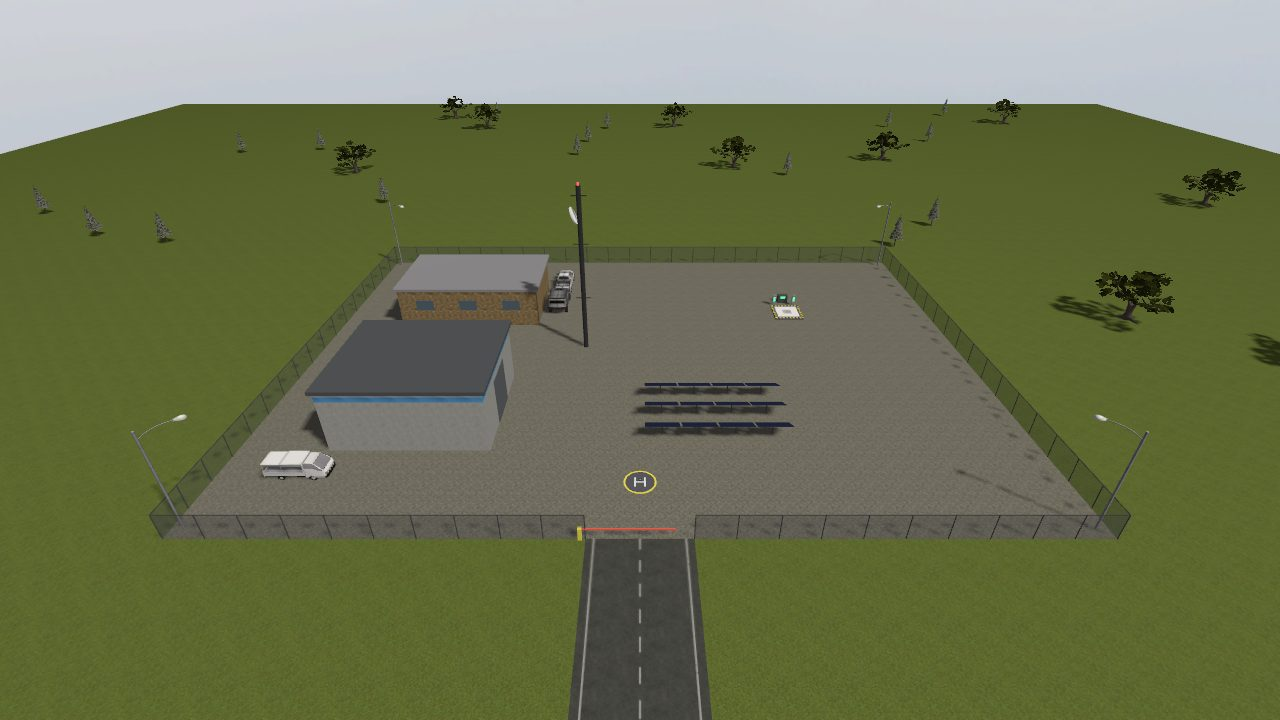
\includegraphics[width=\linewidth]{base_carga}
    \column{0.47\textwidth}\small
    \textbf{Escenario}: un dron de vigilancia patrulla la cerca de una base. Con batería baja, deja la
    patrulla, va a su estación, \textbf{aterriza con precisión} sobre el ArUco 42, ``carga'' y
    \textbf{regresa a patrullar justo donde se quedó}.
    \begin{itemize}
      \item \textbf{Viene de}: \cmd{battery\_monitor} + \cmd{square\_mission}.
    \end{itemize}
  \end{columns}
\end{frame}

\begin{frame}{La batería en PX4 SITL}
  \begin{columns}[c]
    \column{0.47\textwidth}
    \begin{tikzpicture}[x=0.11cm,y=0.025cm]
      \draw[-{Stealth}] (0,0) -- (62,0) node[right,font=\tiny] {s armado};
      \draw[-{Stealth}] (0,0) -- (0,110) node[above,font=\tiny] {\%};
      \draw[azul,thick] (0,100) -- (30,50) -- (40,50);
      \draw[verde,thick] (40,50) -- (40,100) -- (55,75);
      \draw[rojo,dashed] (0,60) -- (60,60) node[right,font=\tiny] {low\_percent};
      \node[font=\tiny,verde] at (40,106) {desarma = 100 \%};
      \node[font=\tiny,azul] at (18,40) {50 \% mínimo};
    \end{tikzpicture}
    \column{0.5\textwidth}\small
    \begin{itemize}
      \item Armado, baja de 100\% a 50\% en 30 s (\cmd{SIM\_BAT\_DRAIN} = 60 s) y \textbf{se queda en 50\%}.
      \item Al \textbf{desarmar} vuelve a 100\% al instante.
      \item O sea: aterrizar en la estación y desarmar \textbf{es cargar}.
      \item \cmd{low\_percent} tiene que ser $> 0.5$ (si no, nunca se dispara).
      \item Se lee de \cmd{/fmu/out/battery\_status\_v1} (\cmd{remaining}, 0--1, a 1 Hz).
    \end{itemize}
  \end{columns}
\end{frame}

\begin{frame}{La patrulla y la máquina de estados}
  \begin{columns}[c]
    \column{0.42\textwidth}\centering
    \begin{tikzpicture}[x=0.042cm,y=0.042cm]
      \draw[gray!50,fill=gray!10] (-35,-6) rectangle (35,46);
      \draw[azul,thick,-{Stealth}] (-31,-2) -- (-31,42) -- (31,42) -- (31,-2) -- (-31,-2);
      \fill[orange] (16.3,28.3) rectangle (19.7,31.7);
      \node[font=\tiny,right] at (20,30) {estación};
      \node[draw,circle,fill=azulclaro,inner sep=0.5pt,font=\tiny] at (0,0) {H};
      \fill[gray!60] (-27,4) rectangle (-13,16); \node[font=\tiny] at (-20,10) {hangar};
    \end{tikzpicture}
    \column{0.55\textwidth}
    \begin{tikzpicture}[node distance=0.22cm,st/.style={draw=azul,fill=azulclaro,rounded corners,font=\tiny,minimum width=1.9cm}]
      \node[st] (p) {PATROL};
      \node[st,right=0.4cm of p] (s) {TO\_STATION};
      \node[st,below=of s,fill=yellow!20] (pr) {PRECISION};
      \node[st,below=of pr] (la) {LANDING};
      \node[st,below=of la] (ch) {CHARGING};
      \node[st,left=0.4cm of ch] (re) {REARM / TAKEOFF};
      \node[st,above=of re] (rs) {RESUME};
      \draw[-{Stealth}] (p) -- node[above,font=\tiny]{batería} (s);
      \draw[-{Stealth}] (s) -- (pr); \draw[-{Stealth}] (pr) -- (la); \draw[-{Stealth}] (la) -- (ch);
      \draw[-{Stealth}] (ch) -- (re); \draw[-{Stealth}] (re) -- (rs); \draw[-{Stealth}] (rs) -- (p);
    \end{tikzpicture}
  \end{columns}
  \vspace{0.3em}
  \small Al dejar la patrulla guarda \textbf{dónde estaba y en qué tramo}; al volver, va ahí primero.
  Patrulla a 8 m y a 4 m de la cerca: lejos del hangar (6.5 m de alto) y la comandancia.
\end{frame}

\begin{frame}{El GPS te lleva cerca; la cámara te pone encima}
  \begin{columns}[c]
    \column{0.47\textwidth}\centering
    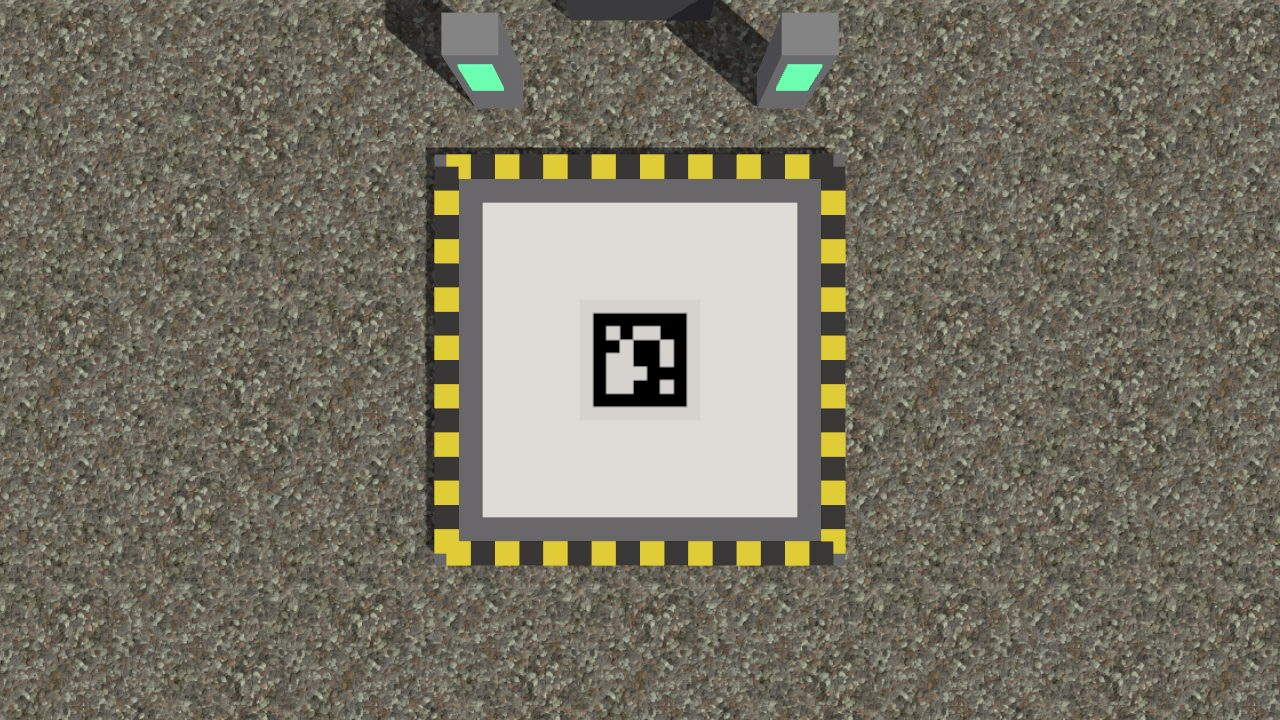
\includegraphics[width=0.9\linewidth]{base_carga_estacion}
    \column{0.5\textwidth}\small
    La estación ``según el mapa'' (\cmd{station\_north/east}) tiene \textbf{1.5 m de error a propósito}:
    la plataforma real está en N 30, E 18.
    \vspace{0.3em}

    \textbf{TODO}: en cada ciclo de la bajada, un setpoint mixto:
    \begin{itemize}
      \item en $x, y$: \textbf{posición} = donde ve el ArUco;
      \item en $z$: \textbf{velocidad} = bajar a \cmd{descent\_speed} solo si ya está \textbf{centrado}
        (\textless 0.2 m); si no, 0 mientras se acomoda;
      \item si no lo ve: quieto y subir un poco para que vuelva a caber en la imagen.
    \end{itemize}
  \end{columns}
\end{frame}

\begin{frame}{Bajar centrado}
  \begin{columns}[c]
    \column{0.45\textwidth}\centering
    \begin{tikzpicture}[scale=0.8]
      \fill[gray!40] (-1.7,0) rectangle (1.7,0.25);
      \fill[black] (-0.35,0.25) rectangle (0.35,0.3);
      \draw[azul,thick,-{Stealth}] (1.5,4) -- (0.3,3.4);
      \draw[azul,thick,-{Stealth}] (0.3,3.4) -- (0,3.1);
      \draw[verde,thick,-{Stealth}] (0,3.1) -- (0,0.9);
      \node[font=\tiny,right] at (1.5,4) {llega por GPS (1.5 m chueco)};
      \node[font=\tiny,right] at (0.35,3.25) {se centra sin bajar};
      \node[font=\tiny,right] at (0.1,2) {baja centrado};
      \draw[rojo,dashed] (-1.8,0.8+0.25) -- (1.8,0.8+0.25) node[right,font=\tiny] {0.8 m: Land};
    \end{tikzpicture}
    \column{0.52\textwidth}\small
    \begin{itemize}
      \item A \textasciitilde0.8 m sobre la plataforma, PX4 termina con \cmd{land()}: detecta el contacto y
        desarma.
      \item \textbf{Éxito}: cada carga aterriza a \textbf{menos de 0.3 m} del centro del ArUco.
      \item Sin el TODO baja derecho sobre la coordenada del mapa y aterriza \textasciitilde1.5 m chueco.
    \end{itemize}
    \begin{terminal}{al terminar}
carga 1: aterrizó a ... m del centro\\
\ \ (máximo 0.3) OK / FALLÓ
    \end{terminal}
  \end{columns}
\end{frame}
